\chapter{Analisis}

\section{Analisis Sistem Kini}

\subsection{Mesin Navigasi KIRI}

KIRI memiliki mesin navigasi yang dibangun pada bahasa Java. Mesin ini bertugas untuk menerima masukan berupa koordinat titik asal dan tujuan, kemudian menemukan angkot-angkot yang harus dinaiki untuk menuju titik tujuan dari titik asal. Karena alasan kerahasiaan, pembahasan mengenai mesin navigasi KIRI tidak mengacu pada referensi publik, melainkan dari survei terhadap kode sumber internal KIRI.

\begin{figure}
	\centering
	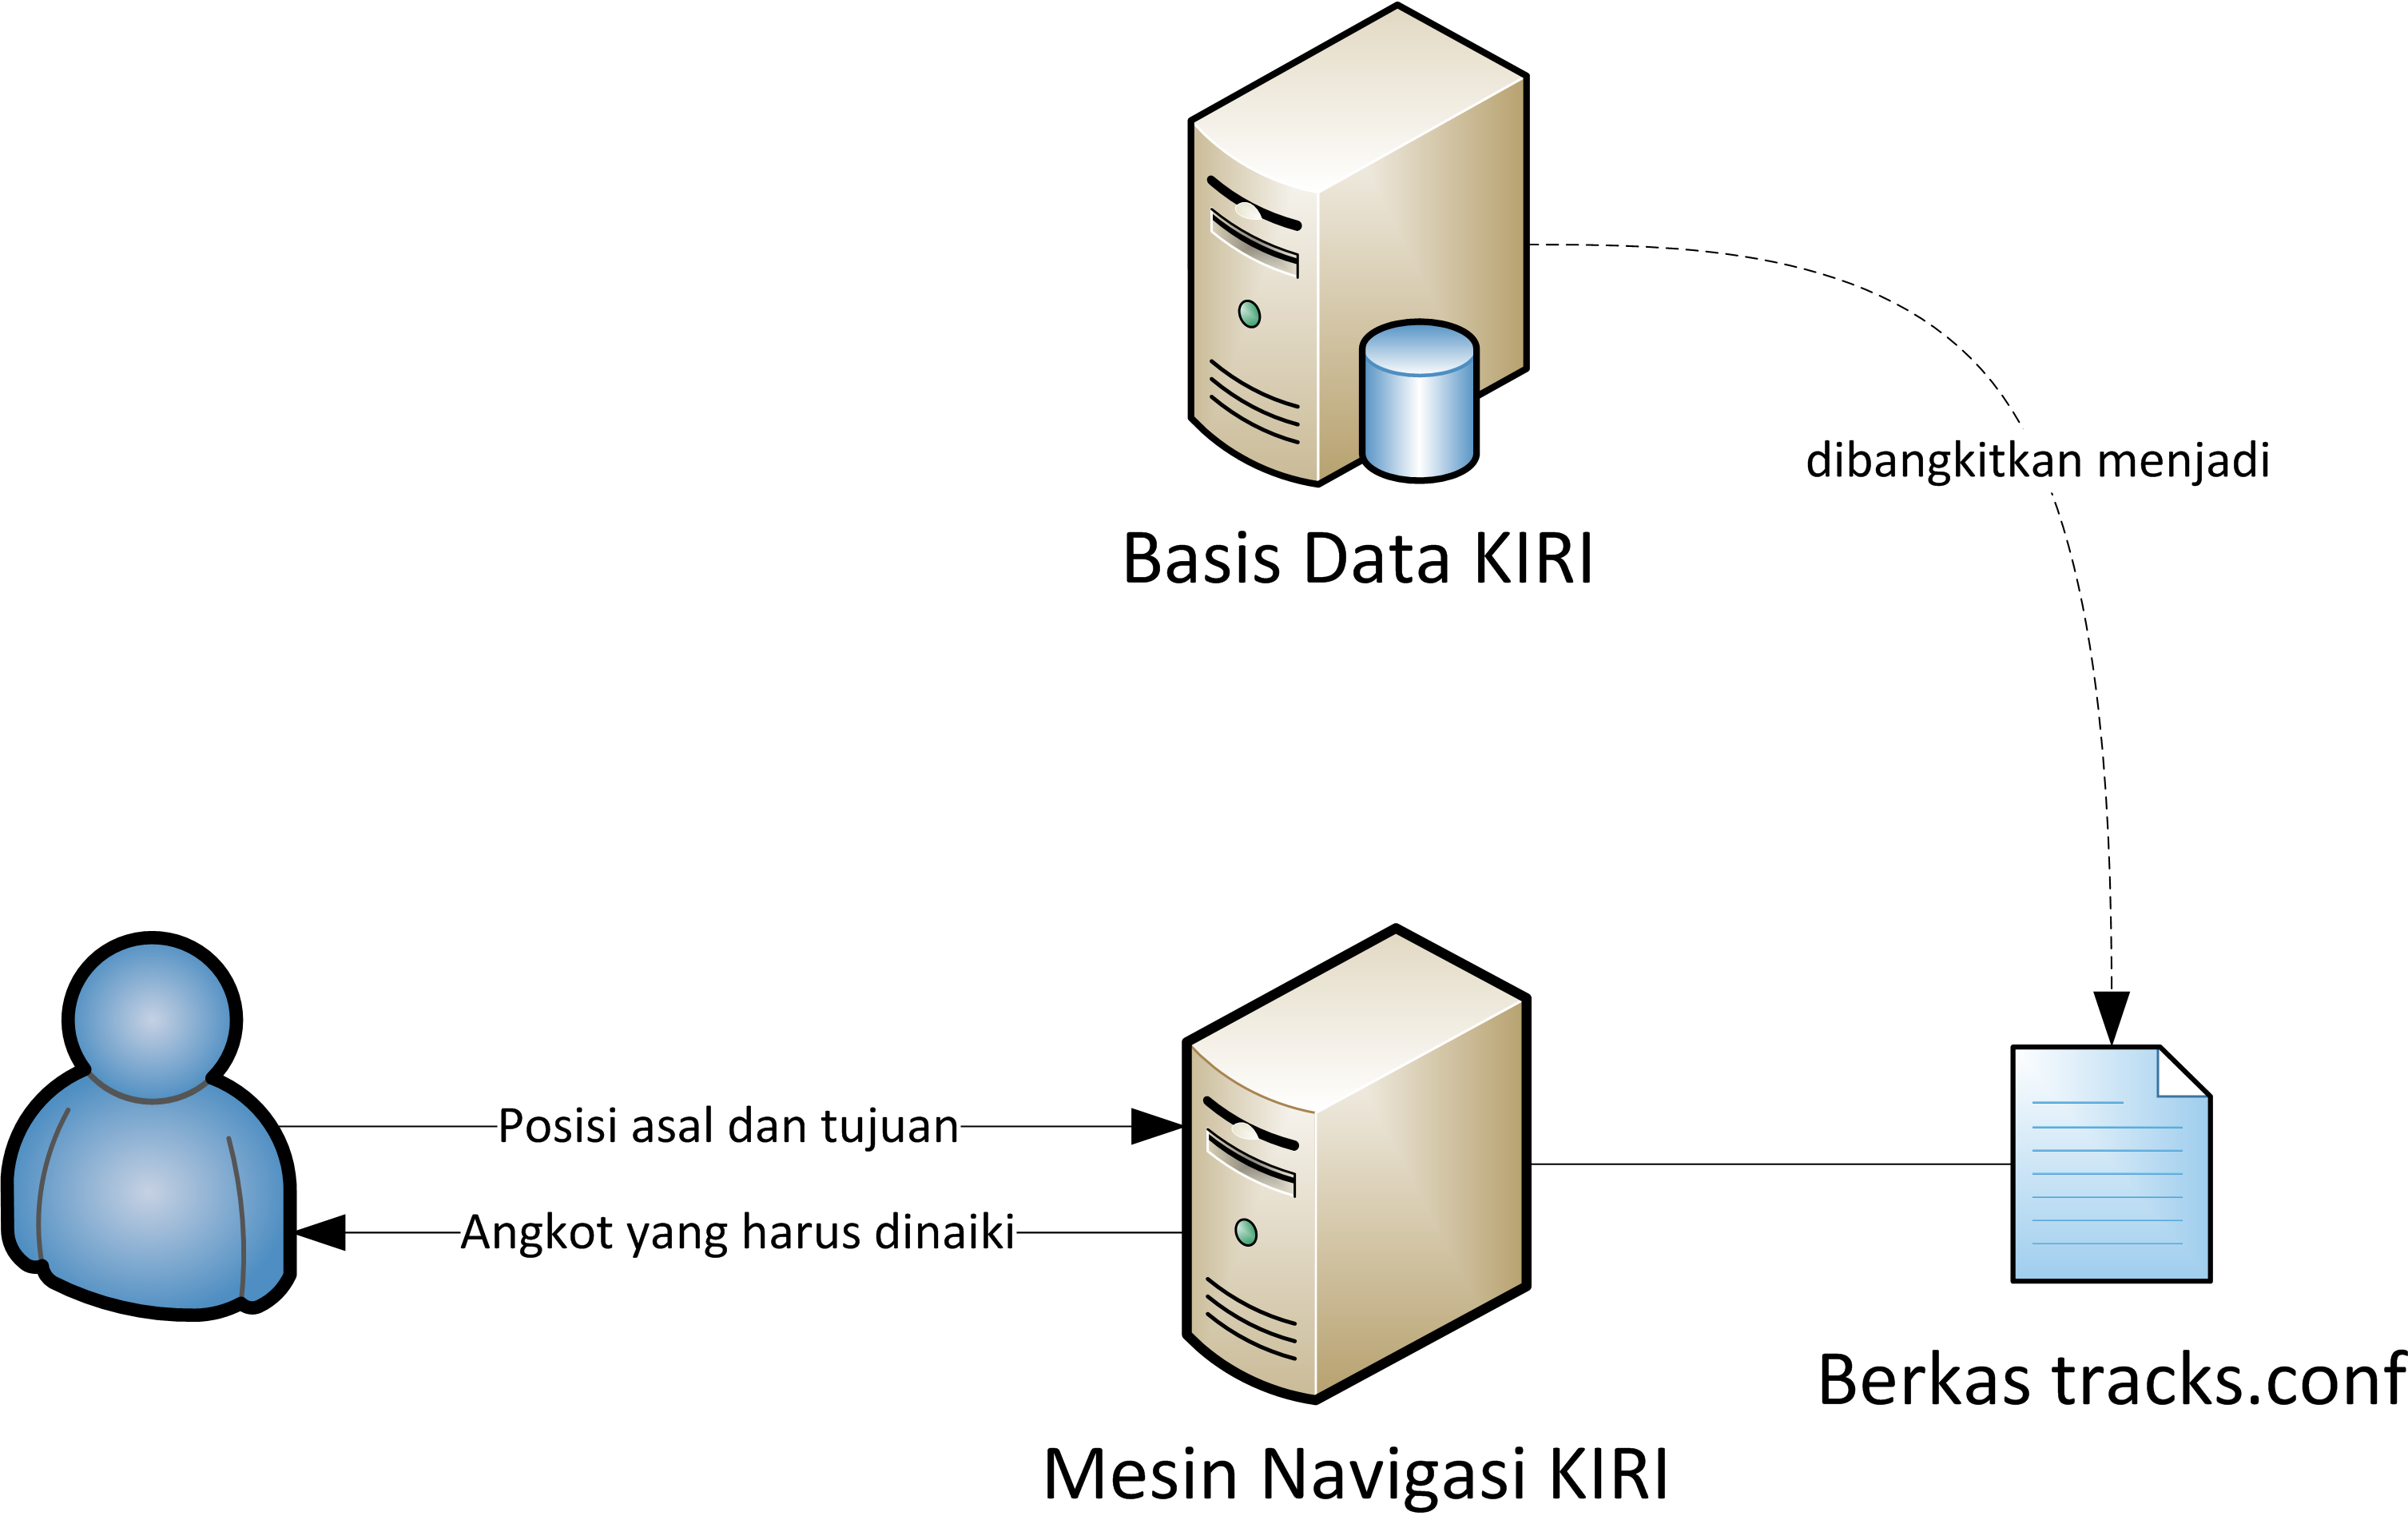
\includegraphics[scale=0.7]{Gambar/2_arsitektur_saat_ini}
	\caption{Arsitektur Saat Ini} 
	\label{fig:2_arsitektur_saat_ini}
\end{figure}

Seperti dapat dilihat pada gambar \ref{fig:2_arsitektur_saat_ini}, elemen
arsitektur yang mendukung navigasi KIRI dibagi menjadi tiga, yaitu:

\begin{enumerate}
	\item \textbf{Basis Data KIRI} menyimpan informasi rute 33 trayek angkot, yang masing-masing mencakup identifikasi trayek (\texttt{trackId} dan \texttt{trackTypeId}), nama trayek (\texttt{trackName}), daftar koordinat yang dilewati (\texttt{geodata}), informasi pulang-pergi (\texttt{pathloop}), catatan internal (\texttt{internalInfo}), prioritas untuk dipilih (\texttt{penalty}), informasi naik/turun penumpang (\texttt{transferNodes}), dan parameter ekstra untuk pembelian tiket (\texttt{extraParameters}).
	\item \textbf{Berkas tracks.conf} adalah hasil ekstraksi dari basis data KIRI, yang menyimpan informasi penting saja yang dibutuhkan oleh algoritma mesin navigasi KIRI, yakni: \texttt{trackId}, \texttt{trackTypeId}, \texttt{penalty}, \texttt{geodata}, \texttt{pathloop}, dan \texttt{transferNodes}.
	\item \textbf{Mesin Navigasi KIRI} adalah program yang bertugas mengolah data yang ada pada berkas tracks.conf, sehingga dapat menjawab pertanyaan navigasi dari titik asal ke titik tujuan. Karena alasan historis, mesin navigasi tidak membaca data langsung dari basis data, melainkan dari berkas tracks.conf.
\end{enumerate}

Ketiga elemen tersebut dijelaskan pada subbab-subbab berikut.

\subsubsection{Basis Data KIRI}
Basis data KIRI disimpan dalam sistem manajemen basis data MySQL. Salah satu dari tabel yang digunakan adalah tabel \texttt{tracks}, yang menyimpan informasi rute trayek. Struktur dari tabel ini dijelaskan pada tabel \ref{tab:2_struktur_tabel_tracks}.

\begin{table}
	\caption{Struktur Tabel tracks}
	\label{tab:2_struktur_tabel_tracks}
	\begin{tabular}{|p{3cm}|p{2.5cm}|p{9.5cm}|}
		\hline
		Nama kolom & Tipe & Keterangan \\
		\hline
		trackId & varchar(32) & Kode trayek angkot (misal: ``\texttt{sthallciumbuleuitlurus}''). Menjadi PRIMARY KEY tabel bersama trackTypeId. \\
		trackTypeId & varchar(32) & Kode tipe trayek (untuk angkot bandung, selalu berisi ``\texttt{bdo\_angkot}''). Menjadi PRIMARY KEY bersama trackId. \\
		trackName & varchar(32) & Nama trayek yang dapat dibaca secara umum (misal: ``\texttt{St. Hall - Ciumbuleuit (lurus)}''). \\
		internalInfo & varchar(1024) & Informasi internal yang dapat ditambahkan dan tidak akan ditampilkan pada hasil pencarian. \\
		geodata & linestring & Daftar koordinat dari rute trayek ini. \\
		pathloop & tinyint(1) & Menandakan apakah trayek ini adalah trayek pulang pergi atau satu arah. \\
		penalty & decimal(4,2) & Bobot dari trayek ini. Semakin besar nilainya, semakin kecil kemungkinan akan muncul pada hasil navigasi. \\
		transferNodes & varchar(1024) & Daftar indeks titik di mana penumpang dapat turun maupun naik, dipisahkan dengan koma. Untuk angkot Bandung, penumpang dapat turun dan naik di semua titik. \\
		extraParameters & varchar(256) & Informasi yang ditambahkan saat melakukan pembelian tiket (tidak terkait dengan penelitian ini). \\
		\hline
	\end{tabular}
\end{table}

\subsubsection{Berkas tracks.conf}
Karena alasan historis\footnote{Pada awalnya mesin navigasi KIRI dibangun menggunakan bahasa C++, sehingga menyulitkan dalam mengakses basis data MySQL}, mesin navigasi KIRI tidak mengakses langsung ke basis data MySQL, melainkan membaca sebuah berkas yang bernama \texttt{tracks.conf}.

Berkas \texttt{tracks.conf} ini merupakan sebuah berkas teks yang menyimpan basis data trayek yang telah dibersihkan untuk dapat dibaca dengan mudah, satu \textit{record} per baris. Setiap baris berisi 6 \textit{field} yang dipisahkan dengan \textit{tab} (\textit{Unicode} U+0009\cite{unicode8}). Berikut adalah penjelasan dari keenam \textit{field} tersebut:

\begin{enumerate}
	\item \textbf{trackTypeId.trackId} Berisi kolom \textit{trackTypeId} dan \textit{trackId} dipisahkan dengan titik.
	\item \textbf{penalty} Berisi nilai kolom \textit{penalty}.
	\item \textbf{numberOfNodes} Berisi jumlah \textit{node} (titik) dari rute trayek ini.
	\item \textbf{nodes} Berisi daftar koordinat \textit{node} dari rute trayek ini dipisahkan dengan \textit{tab}. Setiap koordinat node terdiri dari \textit{latitude} dan \textit{longitude} yang dipisahkan dengan spasi.
	\item \textbf{pathLoop} Berisi nilai kolom \textit{pathloop} yang menunjukkan apakah rute ini merupakan rute pulang pergi atau searah.
	\item \textbf{transferNodes} Berisi nilai kolom \textit{transferNodes} yang menunjukkan titik-titik di mana penumpang diperbolehkan untuk naik atau turun.
\end{enumerate}

\subsubsection{Mesin Navigasi KIRI}

Mesin navigasi KIRI merupakan sebuah program yang mendengarkan dan menjawab permintaan navigasi dalam bentuk \textit{HTTP request} \cite{rfc7231} di \textit{port} 8000. Program ini dibangun di atas bahasa Java, yang terdiri dari beberapa kelas yang ditunjukkan pada gambar \ref{fig:2_diagram_kelas_sistem_kini}.

\begin{figure}
	\centering
	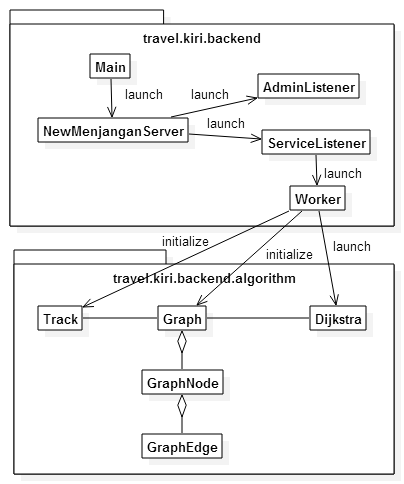
\includegraphics[scale=0.5]{Gambar/2_diagram_kelas_sistem_kini}
	\caption{Diagram Kelas Sistem Kini} 
	\label{fig:2_diagram_kelas_sistem_kini}
\end{figure}

Adapun penjelasan untuk setiap kelas dapat dilihat di bawah ini:

\begin{description}
	\item[Main] Kelas yang berfungsi sebagai antarmuka program, untuk dijalankan dari \textit{console}.
	\item[NewMenjanganServer] Kelas yang bertugas menjalankan program sebagai server, yakni menyiapkan servis-servis untuk dijalankan.
	\item[AdminListener] Kelas yang berfungsi untuk mendengarkan dan merespon perintah administrasi, seperti \textit{ping}, \textit{shutdown}, dll.
	\item[ServiceListener] Kelas yang berfungsi untuk mendengarkan dan merespon permintaan untuk navigasi. Servis ini menerima masukan berupa koordinat asal dan tujuan, dan mengembalikan rute angkot yang harus dinaiki.
	\item[Worker] Kelas ini berfungsi untuk melakukan pekerjaan yang telah diterima oleh ServiceListener. Selain itu, di awal kelas ini juga menyiapkan bahan-bahan yang diperlukan untuk melakukan perhitungan rute, yakni mengkonversi data trayek ke dalam bentuk graf.
	\item[Track] Kelas ini berfungsi untuk menyimpan informasi sebuah trayek angkot beserta rutenya.
	\item[Graph] Kelas ini merepresentasikan sebuah graf.
	\item[GraphNode] Kelas ini merepresentasikan setiap \textit{node} yang dimiliki oleh graf.
	\item[GraphEdge] Kelas ini merepresentasikan sebuah \textit{edge} dari GraphNode.
	\item[Dijkstra] Kelas ini merepresentasikan algoritma \textit{Dijkstra's shortest path}\cite{Cormen:2001}, untuk digunakan dalam pencarian rute.
\end{description}

\subsection{Protokol Peta Angkutan Umum}

Berdasarkan kode sumber Peta Angkutan Umum \cite{angkotwebid}, situs tersebut memanfaatkan \textit{HTTP request} \cite{rfc7231} untuk menerima perintah-perintah dan mengembalikan respon berupa data dalam sintaks JSON. Beberapa dari perintah tersebut dijelaskan pada subbab-subbab berikut.

\subsubsection{Transportation List}
Perintah ini digunakan untuk mendapatkan daftar semua daftar transportasi umum, dan dapat diakses pada dengan melakukan \textit{HTTP request GET} pada path \texttt{/route/transportation-list.json}, tanpa parameter apapun. Adapun kembalian dari perintah ini adalah sebuah objek JSON yang terdiri dari pasangan nama/nilai berikut:

\begin{itemize}
	\item \texttt{status}: Status kembalian dari perintah yang dikirimkan
	\item \texttt{provinces}: \textit{Array} provinsi yang terdaftar, masing-masing elemen merupakan \textit{array} lain yang berisi:
		\begin{itemize}
			\item Kode provinsi
			\item Nama provinsi
		\end{itemize}
	\item \texttt{transportations}: \textit{Array} provinsi yang terdaftar, masing-masing berisi:
		\begin{itemize}
			\item \texttt{hasroute}: Menyatakan apakah trayek ini memiliki data rute
			\item \texttt{company}: Perusahaan pengelola trayek ini
			\item \texttt{id}: Indeks trayek ini dalam basis data
			\item \texttt{origin}: Awal rute trayek
			\item \texttt{destination}: Akhir rute trayek
			\item \texttt{province}: Provinsi tempat trayek ini beroperasi
			\item \texttt{city}: Kota tempat trayek ini beroperasi
			\item \texttt{number}: Nomer trayek
			\item \texttt{created}: \textit{UNIX time} trayek ini dibuat
			\item \texttt{updated}: \textit{UNIX time} trayek ini terakhir diperbaharui
		\end{itemize}
\end{itemize}

Contoh kembalian dari perintah transportation list (\url{https://angkot.web.id/route/transportation-list.json}) dapat dilihat pada kode di bawah ini:

\begin{lstlisting}
{
	"status": "ok",
	"provinces": [
		[
			"ID-AC",
			"Aceh"
		],
		...
	],
	"transportations": [
		{
			"hasRoute": true,
			"company": "KWK",
			"id": 21,
			"origin": null,
			"destination": null,
			"province": "ID-JK",
			"city": "Jakarta",
			"number": "S15A",
			"created": "1379952348",
			"updated": "1379952379"
		},
		...
	]
}
\end{lstlisting}

\subsubsection{Transportation Detail}
Perintah ini digunakan untuk mendapatkan detail dari sebuah trayek transportasi, dan diakses dengan melakukan \textit{HTTP request GET} pada path \texttt{/route/transportation/nnn.json} (di mana \textit{nnn} adalah nomer kode trayek dalam basis data). Adapun kembalian dari perintah ini adalah:

\begin{itemize}
	\item \texttt{id}: Nomer kode trayek.
	\item \texttt{geojson}: Data rute dan atributnya dalam format GeoJSON, terdiri dari:
		\begin{itemize}
			\item \texttt{type}: Tipe GeoJSON yang digunakan, selalu berisi ``\texttt{Feature}''
			\item \texttt{properties}: Properti-properti data GeoJSON, terdiri dari:
				\begin{itemize}
					\item \texttt{number}: Nomer trayek
					\item \texttt{accept}: \textit{tidak diketahui}
					\item \texttt{company}: Perusahaan pengelola trayek ini
					\item \texttt{destination}: Akhir rute trayek
					\item \texttt{province}: Provisi tempat trayek ini beroperasi
					\item \texttt{origin}: Awal rute trayek
					\item \texttt{city}: Kote tempat trayek ini beroperasi
				\end{itemize}
			\item \texttt{properties}: Data geometri rute trayek ini, mengikuti standar GeoJSON untuk tipe data \texttt{MultiLineString}.
		\end{itemize}
	\item \texttt{created}: \textit{UNIX time} trayek ini dibuat
	\item \texttt{status}: Status kembalian dari perintah yang dikirimkan
	\item \texttt{submission\_id}: Kode submisi dari trayek yang dimaksud
	\item \texttt{updated}: \textit{UNIX time} trayek ini terakhir diperbaharui
\end{itemize}

Contoh kembalian dari perintah transportation (https://angkot.web.id/route/transportation/348.json) dapat dilihat pada kode berikut:

\begin{lstlisting}
{
	"id": 348,
	"geojson": {
		"type": "Feature",
		"properties": {
			"number": "M24v2",
			"accept": [],
			"company": "Mikrolet",
			"destination": "Joglo",
			"province": "ID-JK",
			"origin": "Terminal Grogol",
			"city": "Jakarta"
		},
		"geometry": {
			"type": "MultiLineString",
			"coordinates": [
				[
					[106.79068207740782, -6.166144969433212],
					[106.79347157478333, -6.166107635752627],
					[106.79707646369934, -6.165899633769797],
					...
				],
				[
					[106.7961323261261, -6.196021736671819],
					[106.7957353591919, -6.196037735916297],
					[106.79550468921661, -6.195936407359816],
					...
				]
			]
		}
	},
	"created": "1402504737",
	"status": "ok",
	"submission_id": "CaZVRi",
	"updated": "1402506397"
}
\end{lstlisting}




\section{Analisis Sistem Usulan}

\subsection{Mesin Navigasi KIRI}

\subsubsection{Mekanisme Penarikan}

Untuk mendukung integrasi data antara Peta Angkutan Umum dan KIRI, diperlukan adanya penarikan secara berkala terhadap Peta Angkutan Umum oleh KIRI. Ada dua alternatif metode yang dipertimbangkan sebagai mekanisme penarikan data ini:

\begin{description}
	\item \textbf{Metode \textit{realtime}} mendeteksi setiap perubahan yang terjadi pada data Peta Angkutan Umum, dan langsung memberi notifikasi kepada KIRI untuk mengambil ulang data yang berubah dari Peta Angkutan Umum
	\item \textbf{Metode \textit{polling}} di mana KIRI akan mengambil data secara berkala dari Peta Angkutan Umum, sehingga akan terdapat jeda antara perubahan data dan terbaharuinya data KIRI.
\end{description}

Dari kedua metode tersebut, metode \textit{polling} dipilih dengan alasan-alasan sebagai berikut:

\begin{itemize}
	\item \textbf{Lebih sedikit perubahan} Peta Angkutan Umum menggunakan protokol HTTP yang bersifat \textit{conectionless}, sehingga secara alami akan menunggu perintah dari \textit{client}, alih-alih secara aktif memberi notifikasi kepada \textit{client}. Jika menggunakan metode \textit{polling}, KIRI dapat memanfaatkan protokol \textit{Transportation Detail} yang sudah dimiliki oleh Peta Angkutan Umum.
	\item \textbf{Mengurangi kebutuhan prosesor} Rute pada KIRI dimodelkan dalam bentuk graf, dan sebelum dapat digunakan untuk pencarian graf ini harus dikonstruksi terlebih dahulu. Akibat besarnya data yang digunakan, konstruksi ini akan memakan waktu (kurang lebih 30 detik). Dengan menggunakan metode \textit{realtime}, setiap perubahan data pada kiri.web.id akan mengakibatkan graf ini harus direkonstruksi ulang. Dengan menggunakan metode \textit{polling}, penarikan data dan rekonstruksi graf dapat dijadwalkan sedemikian sehingga dilakukan pada saat pengguna sedang tidak aktif.
	\item \textbf{Urgensi Perbaikan Data} Urgensi perbaikan data tidak terlalu tinggi untuk KIRI (jika dibandingkan dengan perubahan harga saham, \textit{realtime GPS monitoring}, dll) sehingga penarikan tidak perlu dilakukan terlalu sering.
\end{itemize}

Ditetapkan penggunaan metode \textit{polling} selama 24 jam sekali, dan dipilih waktu 0.30 (setengah jam setelah tengah malam) untuk melakukan \textit{polling}. Penetapan waktu ini mempertimbangkan sedikitnya penggunaan KIRI pada saat tengah malam. Jeda setengah jam dilakukan untuk memberikan toleransi terhadap perbedaan waktu komputer beberapa detik, yang mungkin memberikan masalah pada tanggal sistem. 

\subsubsection{Penyimpanan Data}

Penyimpanan data diusahakan untuk meminimalisir perubahan serta menjaga kompatibilitas dengan versi sebelumnya. Seperti yang telah dibahas pada bab 2, mesin navigasi KIRI menggunakan berkas \texttt{tracks.conf} sebagai jembatan dari basis data menuju mesin navigasi. Berkas inilah yang akan dikonstruksi menjadi graf oleh kelas \texttt{Worker}. Peneliti memutuskan untuk tidak mengubah format dari berkas ini, melainkan melakukan modifikasi pada basis data.

Pada basis data, tetap diusahakan untuk meminimalisir perubahan. Dari struktur tabel \texttt{tracks} yang digunakan, diidentifikasi bahwa kolom \texttt{internalInfo} tidak digunakan dalam perhitungan (tidak berpengaruh pada konstruksi graf). Oleh sebab itu, kolom ini menjadi kandidat untuk disisipkan informasi terkait dengan penarikan data dari Peta Angkutan Umum. Adapun informasi yang harus disimpan adalah:

\begin{itemize}
	\item Penanda bahwa rute ini ditarik dari Peta Angkutan Umum.
	\item Kode yang mengacu pada basis data Peta Angkutan Umum, dalam hal ini \texttt{id}.
\end{itemize}

\subsubsection{Analisis Aplikasi}

Pada penelitian ini, mesin navigasi KIRI dimodifikasi dengan menambahkan dua kelas baru, yaitu kelas \texttt{DataPuller} yang difungsikan sebagai penarik data dari Peta Angkutan Umum, serta kelas \texttt{DataPullerException} untuk mencatat kesalahan pada saat menarik data dari Peta Angkutan Umum. Kelas-kelas yang baru serta yang lama digambarkan pada diagram kelas di gambar \ref{fig:3_diagram_kelas_sistem_usulan}.

\begin{figure}
	\centering
	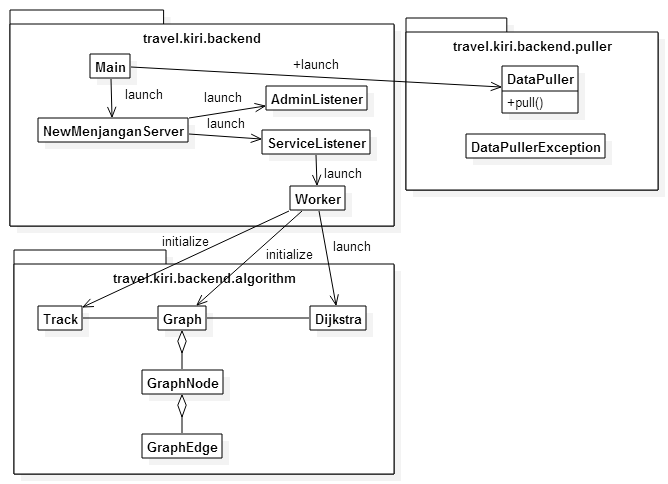
\includegraphics[scale=0.5]{Gambar/3_diagram_kelas_sistem_usulan}
	\caption{Diagram Kelas Sistem Usulan (Tahap Analisis)} 
	\label{fig:3_diagram_kelas_sistem_usulan}
\end{figure}

\subsection{Peta Angkutan Umum}

Pada dasarnya Peta Angkutan Umum tidak diperlukan adanya perubahan, karena KIRI dapat memanfaatkan protokol \textit{transportartion detail}. Namun, untuk keperluan optimasi, ada sedikit perubahan yang dijelaskan pada subbab berikutnya.

\subsection{Optimasi}

Dengan mekanisme yang sudah dijelaskan di subbab sebelumnya, data pada KIRI dapat tersinkronisasi dengan Peta Angkutan Umum. Namun, mekanisme tersebut dirasa tidak optimal. Setiap pukul 0.30, KIRI akan menarik ke-33 rute angkot yang dicatat pada Peta Angkutan Umum, terlepas dari apakah ada perubahan pada rute angkot atau tidak. Walaupun hanya menarik 33 rute dan dilakukan pada jam tidak sibuk, peneliti merasa optimasi tetap dibutuhkan sehingga solusi ini skalabel.

Mekanisme \textit{Transportation List} maupun \textit{Transportation Detail} pada Peta Angkutan Umum memberikan informasi \textit{updated} yang menunjukkan waktu terakhir rute ini diperbaharui. Pada saat menarik data dari Peta Angkutan Umum, informasi ini dapat dicatat dan disimpan pada basis data, untuk dibandingkan pada kesempatan berikutnya. Jika informasi \textit{updated} yang terdapat pada basis data sama atau lebih baru dibandingan dengan yang didapat dari Peta Angkutan Umum, maka tidak diperlukan adanya penarikan rute dari Peta Angkutan Umum. Adapun informasi yang dicatat pada basis data KIRI menjadi sebagai berikut (informasi baru hasil optimasi \textbf{dicetak tebal}):

\begin{itemize}
	\item Penanda bahwa rute ini ditarik dari Peta Angkutan Umum
	\item Kode yang mengacu pada basis data Peta Angkutan Umum, dalam hal ini \texttt{id}.
	\item \textbf{Waktu terakhir rute ini berubah pada Peta Angkutan Umum}
\end{itemize}

Perlu dicatat pula bahwa tidak semua data trayek di Peta Angkutan Umum akan diintegrasikan dengan KIRI. Oleh karena itu, dibutuhkan sedikit perubahan pada Peta Angkutan Umum, sehingga KIRI dapat menarik informasi untuk rute-rute yang dibutuhkan saja. Detail dari perubahan ini akan dijelaskan pada bab berikutnya.